%! Author = nadutkinfedor
%! Date = 04.01.2024

% Preamble
\documentclass[11pt]{article}
\usepackage[left=2cm, right=1cm, top=2cm, bottom=2cm, bindingoffset=0cm]{geometry}

% Packages
\usepackage[utf8]{inputenc}
\usepackage[russian]{babel}
\usepackage{amsmath}
\usepackage{hyperref}
\usepackage{graphicx}
\usepackage{misccorr}
\usepackage{listings}
\usepackage{xcolor}
\usepackage{titlesec}
\usepackage{minted}
\usepackage{color}
\usepackage{enumitem}

%listing settings
\definecolor{dkgreen}{rgb}{0,0.6,0}
\definecolor{gray}{rgb}{0.5,0.5,0.5}
\definecolor{mauve}{rgb}{0.58,0,0.82}

\lstset{language=SQL,
    basicstyle={\small\ttfamily},
    belowskip=3mm,
    breakatwhitespace=true,
    breaklines=true,
    classoffset=0,
    columns=flexible,
    commentstyle=\color{dkgreen},
    framexleftmargin=0.25em,
    keywordstyle=\color{blue},
    numbers=none, %If you want line numbers, set `numbers=left`
    numberstyle=\tiny\color{gray},
    showstringspaces=false,
    stringstyle=\color{mauve},
    tabsize=3,
    xleftmargin =1em,
    backgroundcolor=\color{gray!10}
}

\lstset{ %
    backgroundcolor=\color{white},   % choose the background color
    basicstyle=\footnotesize,        % size of fonts used for the code
    breaklines=true,                 % automatic line breaking only at whitespace
    captionpos=b,                    % sets the caption-position to bottom
    commentstyle=\color{dkgreen},    % comment style
    escapeinside={\%*}{*},          % if you want to add LaTeX within your code
    keywordstyle=\color{blue},       % keyword style
    stringstyle=\color{mauve},     % string literal style
}

% Title
\title{DB internals. Первая лекция}
\author{Надуткин Федор }
\date{December 2023}

\titleformat{\section}[block]{\Huge\bfseries\filcenter}{}{1em}{}
\titleformat{\subsection}[block]{\huge\bfseries\filcenter}{}{1em}{}
\titleformat{\subsubsection}[block]{\Large\bfseries\filcenter}{}{1em}{}

% Document
\begin{document}
    \maketitle

    \newpage

    \section*{Основы реляционной алгебры}

    \textbf{Тип данных} --- описание множества возможных значений какой-либо величины и допустимых операций.

    \begin{itemize}
        \item Логический тип (\texttt{bool}).
        \item Числовые типы (\texttt{int}, \texttt{bigint}, \texttt{float}).
        \item Строковые (\texttt{char}, \texttt{varchar}).
        \item Дата и время (\texttt{date}, \texttt{timestamp}, \ldots).
        \item Контейнеры (\texttt{array}, \texttt{map}).
        \item Специальные типы (\texttt{binary}, \texttt{json}, \texttt{spatial}, \ldots)
    \end{itemize}

    \textbf{Атрибут} --- пара <имя, тип>

    Пример:
    \begin{itemize}
        \item name: \texttt{varchar}
        \item age: \texttt{int}
    \end{itemize}

    \textbf{Значение атрибута} --- величина, принадлежащая типу атрибута

    Пример:
    \begin{itemize}
        \item name: \texttt{varchar}: John
        \item age: \texttt{int}: 30
    \end{itemize}

    \textbf{Кортеж(tuple)} --- несортированное множество атрибутов и их значений

    Пример:
    \begin{itemize}
        \item \text{[} name:\texttt{varchar}:John, age:\texttt{int}:30 \text{]}
    \end{itemize}

    \textbf{Отношение(relation)} - несортированный набор кортежей.
    Отношение может содержать повторяющиеся кортежи

    \begin{center}
        \begin{tabular}{| c | c |}
            \hline
            \textbf{name:varchar} & \textbf{age: int} \\
            \hline
            John                  & 30                \\
            \hline
            Jake                  & 25                \\
            \hline
            John                  & 30                \\
            \hline
        \end{tabular}
    \end{center}

    \newpage

    \textbf{Эквивалентные отношения}
    \begin{itemize}
        \item Одинаковый набор кортежей.
        \item Два кортежа равны, если они содержат идентичный набор атрибутов, и каждая пара одинаковых атрибутов имеет одинаковые значения.
    \end{itemize}

    \textbf{Реляционные оператор} --- функция, которая принимает ноль/одно/несколько отношений и возвращает ноль или одно отношение.

    \includegraphics*[width=0.7\textwidth]{Pictures/Relational algebra/Relational operator}

    \subsection*{Синтаксический анализ}

    \begin{figure}[h!]
        \begin{minipage}{0.4\textwidth}
            \begin{lstlisting}[language=SQL,
                label={lst:sql_syntax_analysis},
                caption={Пример кода}]
                SELECT dept.name, COUNT (* )
                FROM emp, dept
                WHERE
                emp.dept_id = dept.id
                GROUP BY dept. name
            \end{lstlisting}
        \end{minipage}%
        \begin{minipage}{0.7\textwidth}
            \centering
            \includegraphics*[width=0.7\textwidth]{Pictures/Relational algebra/Syntax analysis}
            \caption{Дерво разбора}
        \end{minipage}
        \label{fig:syntax_anlysis}
    \end{figure}

    \textbf{Задача:} Проверка, что запрос сформулирован правильно, согласно правилам запроса.

    \textbf{Результат:} Синтаксическое дерево, если запрос сформулирован верно.
    Ошибка (зачастую достаточно точная), если запрос сформулирован неверно.

    \textbf{Примеры:}
    \begin{itemize}
        \item Postgres/Bison
        \item Trino/ANTLR
    \end{itemize}

    \subsection*{Семантический анализ}

    \begin{figure}[h!]
        \centering
        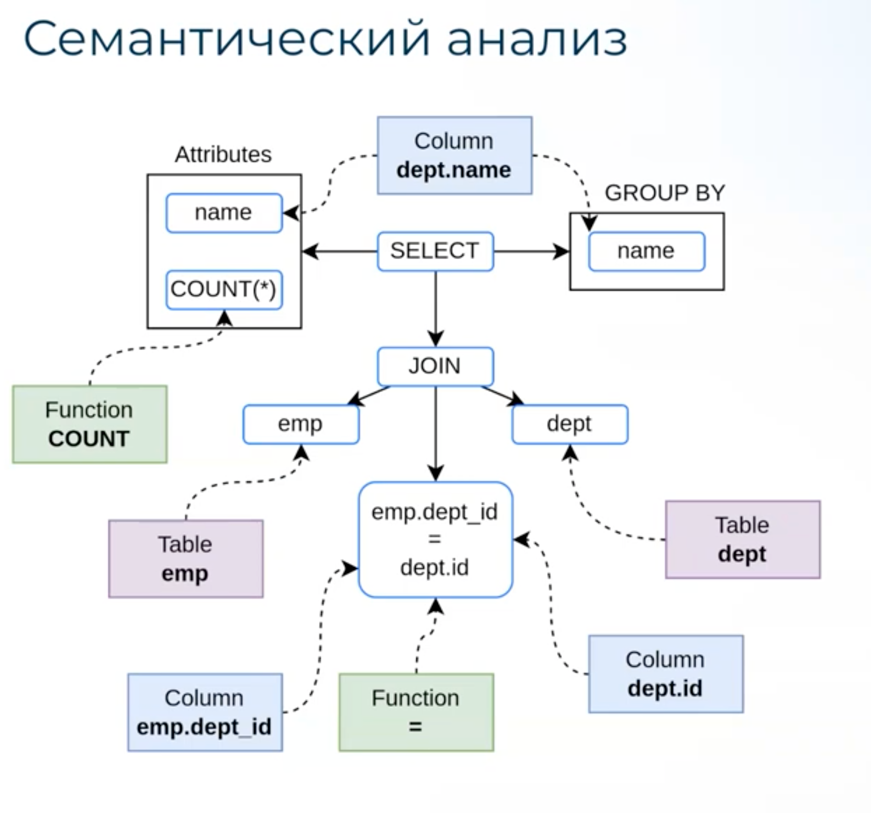
\includegraphics[width=0.6\textwidth]{Pictures/Relational algebra/Semantic analysis}
        \caption{Пример семантического анализа}
    \end{figure}

    Проверяет логическую корректность запроса:
    \begin{itemize}
        \item Доступность объектов
        \item Семантика операторов
    \end{itemize}
    Обычно реализован в виде монолитного компонента, специфичного для конкретного движка.

    \subsection*{Оптимизация}

    \subsubsection*{Оптимизация на основе AST}

    Некоторые движки (как например Postgres) реализуют планирование запросов на основе синтаксического дерева (или схожего представления).
    \begin{itemize}[label=+]
        \item Быстро рекализуют некоторые оптимизации.
    \end{itemize}
    \begin{itemize}[label=-]
        \item Ограничивает потенциал оптимизатора из-за сложно структуры синтаксического дерева.
    \end{itemize}

    \newpage

    \subsubsection*{Оптимизация на основе реляционного представления}

    \begin{figure}[h!]
        \centering
        \vspace{1cm}
        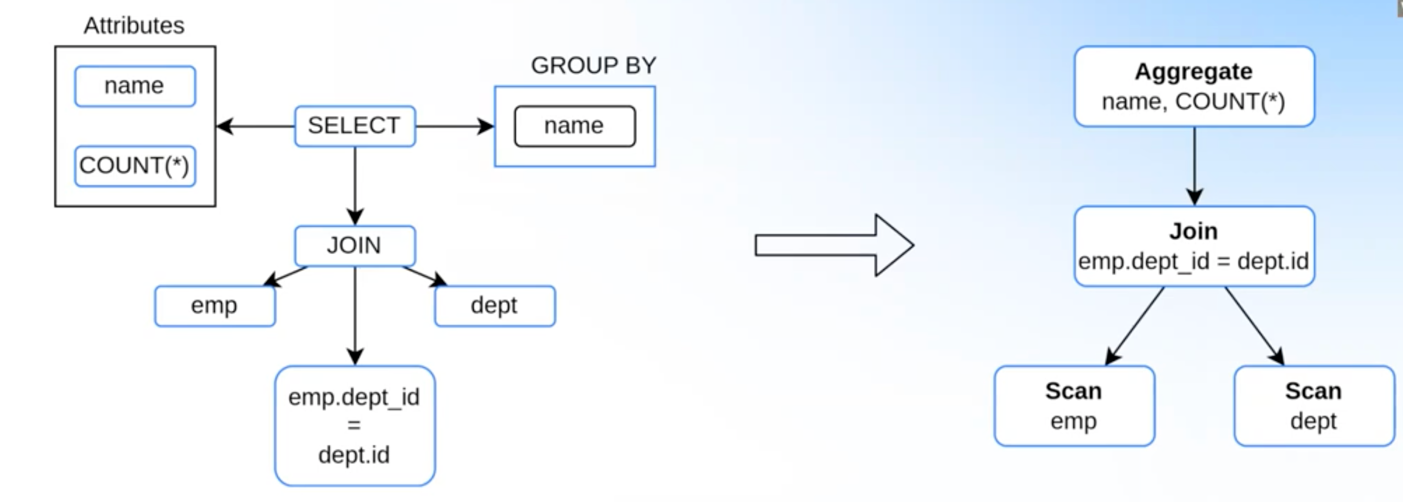
\includegraphics[width=0.6\textwidth]{Pictures/Relational tree}
        \caption{Трансформация в реляционное дерево}
    \end{figure}

    В реляционном предствалении операторы имеют простую семантику (\texttt{Scan}, \texttt{Project}, \texttt{Filter}, \texttt{Join}, \ldots),
    что позволяет реализовывать более широкий спектр трансформаций.
    Зачастую этот процесс происходит в ходе семантического анализа.

    \texttt{Note:} Postgres трансформируется в реляционное дерево уже после оптимизации.

    \newpage


    \section{Row expressions}

    \begin{figure}[h!]
        \begin{minipage}{0.4\textwidth}
            \begin{lstlisting}[language=SQL,
                caption={Пример кода}]
                dept = 'HR'
                AND salary > 100
            \end{lstlisting}
        \end{minipage}
        \begin{minipage}{0.6\textwidth}
            \centering
            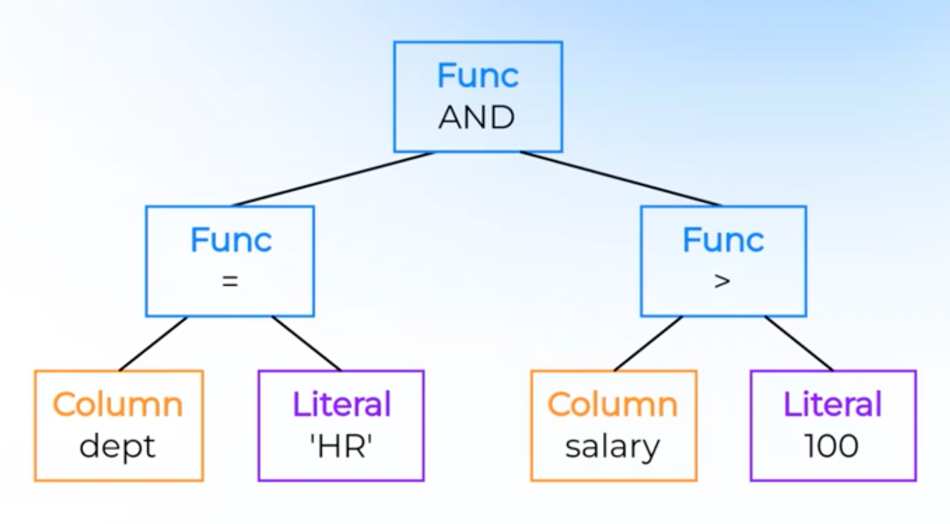
\includegraphics[width=0.9\textwidth]{Pictures/Row expressions}
            \caption{Пример разбора}
        \end{minipage}
    \end{figure}

    \textbf{Row expression} --- дерево выражений, которое возвращает одно значение.
    Вход и выходы -- конкретные значения.

    \begin{lstlisting}[language=Java,
        caption={Интерфейс Row expression}]
            interface RowExpression {
                Type getType ();
                T accept (Visitor<T> visitor);
                boolean equals ();
                int hashCode ();
            }
    \end{lstlisting}

    \textbf{Константа} --- терминальный узел, который содержит типизированное значение.

    \begin{lstlisting}[language=Java,
        caption={Класс константы}]
        class Literal implements RowExpression {
            Object value;
            Type type;
        }
    \end{lstlisting}

    \textbf{Атрибут} --- терминальный узел, который ссылается на значение в атрибуте текущего кортежа.

    Есть 2 способа представления атрибута.

    \begin{itemize}
        \item Адресация происходит по имени, порядок атрибутов в отношении не имеет значения.
        \begin{lstlisting}[language=Java,
            caption={Пример адресации по имени}]
            class Column implements RowExpression {
                String name;
                Type type;
            }
        \end{lstlisting}
        \item Адресация происходит по индексу, порядок атрибутов в отношении имеет значение.
        \begin{lstlisting}[language=Java,
            caption={Пример адресации по индексу}]
            class Column implements RowExpression {
                int index;
                Type type;
            }
        \end{lstlisting}
    \end{itemize}

    \textbf{Функция} --- промежуточный узел, который содержит вызываемую функцию и аргументы.

    \begin{lstlisting}[language=Java,
        caption={Функция}]
        class Call implements RowExpression {
            Function descriptor;
            Type type;
            List<RowExpression> arg;
        }
    \end{lstlisting}

    \newpage


    \section{Реляционные операторы}

    \subsection{Scan}

    \begin{figure}[h!]
        \begin{minipage}{0.4\textwidth}
            \begin{lstlisting}[language=SQL, caption={SQL приводящий в Scan}]
                SELECT city, amount
                FROM sales
                WHERE city = 'SPB'
            \end{lstlisting}
        \end{minipage}
        \begin{minipage}{0.6\textwidth}
            \centering
            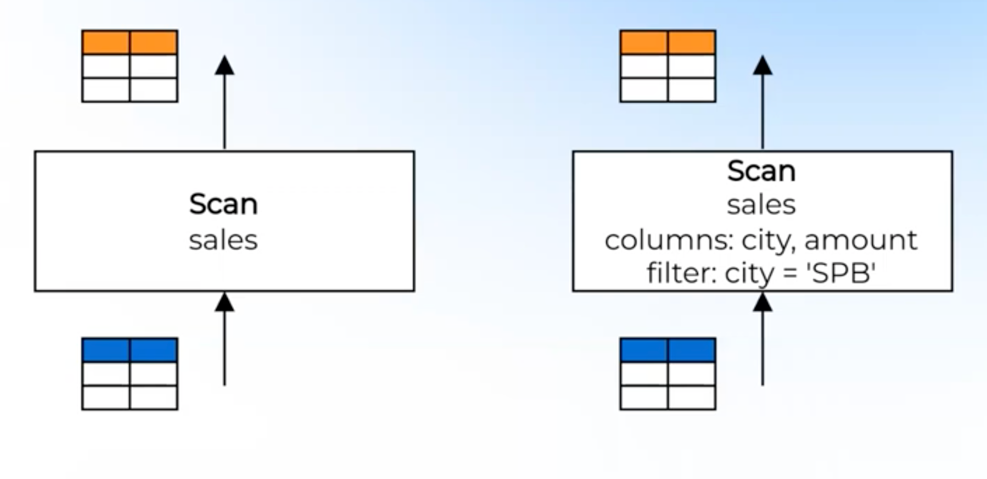
\includegraphics[width=\textwidth]{Pictures/Operators/Scan}
            \caption{Работа Scan}
        \end{minipage}
    \end{figure}

    \textbf{Scan} --- листовой оператор, который возвращает данные из какого-либо источника.

    \begin{itemize}
        \item Всегда содержит ссылку на объект сканирования.
        \item Может опционально содержать стратегию доступа к объекту.
        \item Может содержать дополнительную инормацию для оптимизации процедуры сканирования.
        (Колонки которые надо сканировать, дополнительные фильтры)
    \end{itemize}

    \newpage

    \subsection{Project}

    \begin{figure}[h!]
        \begin{minipage}{0.4\textwidth}
            \begin{lstlisting}[language=SQL, caption={SQL приводящий в Project}]
                SELECT
                city,
                amount * comission as 'agent pay'
                FROM sales
            \end{lstlisting}
        \end{minipage}
        \begin{minipage}{0.6\textwidth}
            \centering
            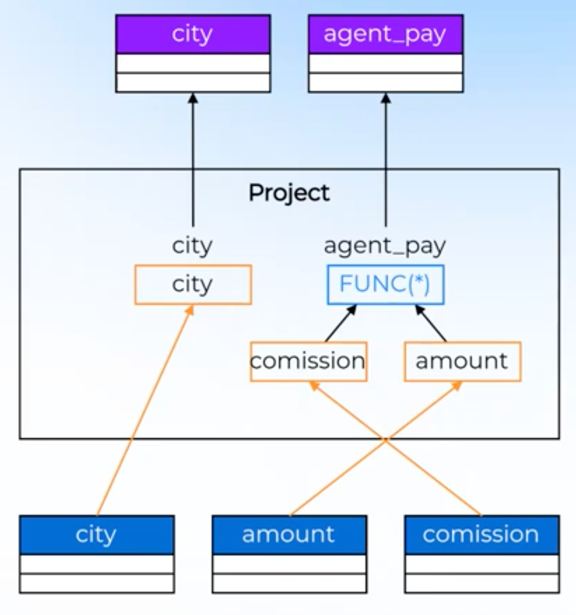
\includegraphics[width=0.6\textwidth]{Pictures/Operators/Project}
            \caption{Работа Project}
        \end{minipage}
    \end{figure}

    \textbf{Project} --- промежуточный оператор, формирующий из входного кортежа, новый кортеж с неким другим набором атрибутов при помощи коллекции \textbf{row expression}.

    \newpage

    \subsection{Filter}

    \begin{figure}[h!]
        \begin{minipage}{0.4\textwidth}
            \begin{lstlisting}[language=SQL, caption={SQL приводящий в Filter}]
                SELECT city, amount
                FROM sales
                WHERE city = 'SPB'
            \end{lstlisting}
        \end{minipage}
        \begin{minipage}{0.6\textwidth}
            \centering
            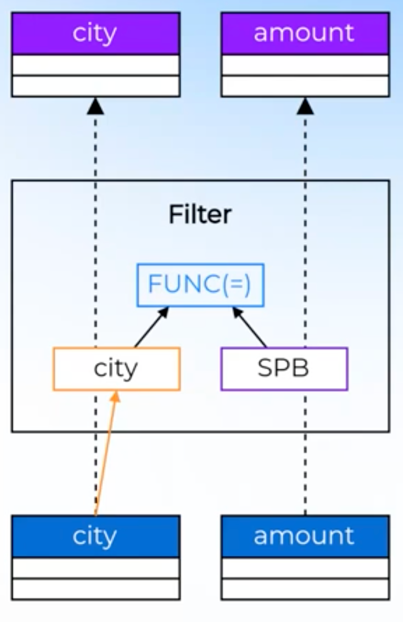
\includegraphics[width=\textwidth]{Pictures/Operators/Filter}
            \caption{Работа Filter}
        \end{minipage}
    \end{figure}

    \textbf{Filter} --- промежуточный оператор, который отфильтровывает определённые кортежи, не удовлетворяющие предикату (некоему \textbf{row expression}).

    \newpage

    \subsection{Aggregation}

    \begin{figure}[h!]
        \begin{minipage}{0.4\textwidth}
            \begin{lstlisting}[language=SQL, caption={SQL приводящий в Aggregation}]
                SELECT year, city, SUM(amount)
                FROM sales
                GROUP BY ROLLUP year, city
            \end{lstlisting}
        \end{minipage}
        \begin{minipage}{0.6\textwidth}
            \centering
            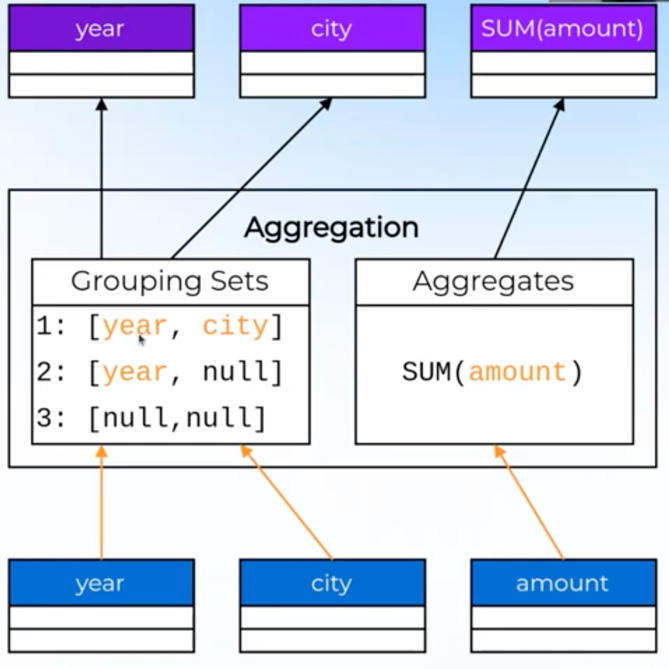
\includegraphics[width=\textwidth]{Pictures/Operators/Aggregation}
            \caption{Работа Aggregation}
        \end{minipage}
    \end{figure}

    \textbf{Aggregation} --- промеждуточный оператор, который считает \textbf{Aggregates} по \textbf{Grouping Sets}.

    \newpage

    \subsection{Sort}

    \begin{figure}[h!]
        \begin{minipage}{0.4\textwidth}
            \begin{lstlisting}[language=SQL, caption={SQL приводящий в Sort}]
                SELECT year, city
                FROM sales
                ORDER BY year ASC, city DESC
            \end{lstlisting}
        \end{minipage}
        \begin{minipage}{0.6\textwidth}
            \centering
            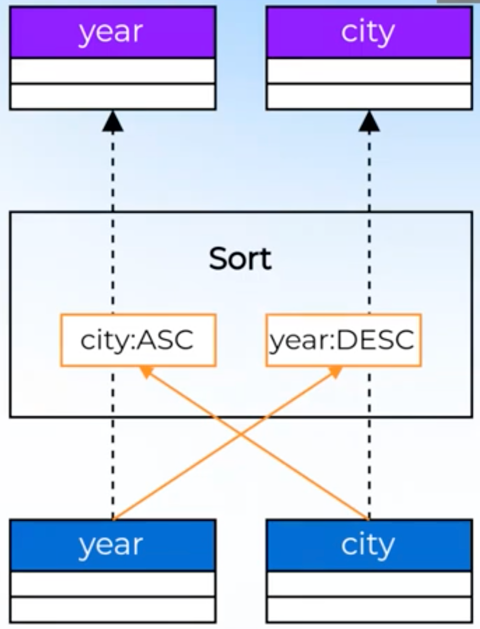
\includegraphics[width=\textwidth]{Pictures/Operators/Sort}
            \caption{Работа Sort}
        \end{minipage}
    \end{figure}

    \textbf{Sort} --- промежуточный оператор, меняющий порядок кортежей.
    С точки зрения SQL, имеет смысл для отображения результата, только конечному пользователю, так как обычно порядок не важен в отношениях.
    Может быть добавлен в обход пользователя (например для merge join) для будущих оптимизаций.

    \newpage

    \subsection{Join}

    \begin{figure}[h!]
        \begin{minipage}{0.4\textwidth}
            \begin{lstlisting}[language=SQL, caption={SQL приводящий в Join}]
                SELECT city_id, amount, id, name
                FROM sales JOIN city
                ON sales.city id = city.id
            \end{lstlisting}
        \end{minipage}
        \begin{minipage}{0.6\textwidth}
            \centering
            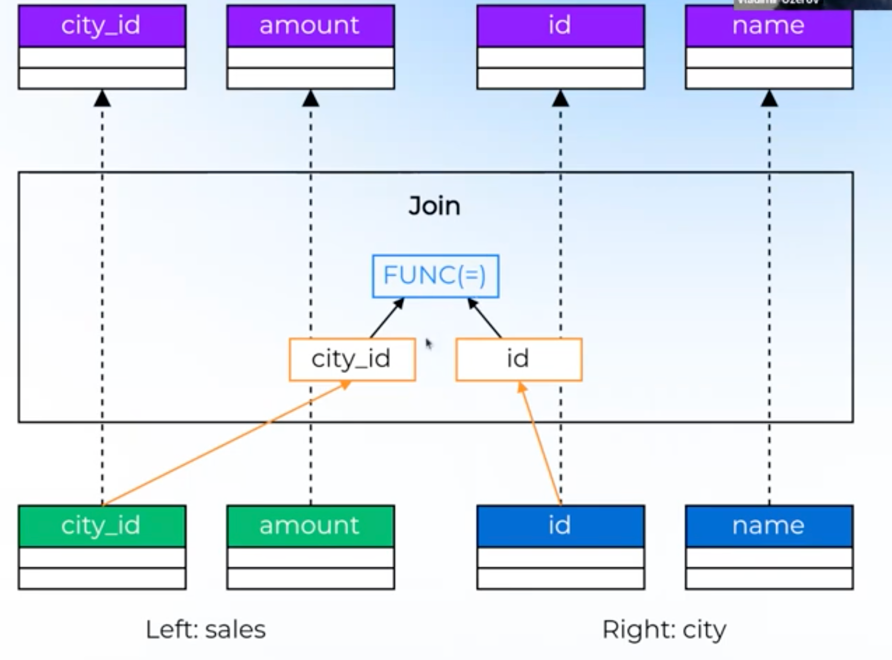
\includegraphics[width=\textwidth]{Pictures/Operators/Join}
            \caption{Работа Join}
        \end{minipage}
    \end{figure}

    \textbf{Join} --- промежуточный оператор, который соединяет данные с нескольких входов по условию.
    \textbf{On} -- по факту является неким предикатом, соединяющим нужные записи и отфильтровывающий не удовлетворяющие условию кортежи.
    Зачастую бинарный из-за простоты имплементации, но могут быть множественными (а также может переводить в множественный и оптимизировать начиная от него).

    \newpage

    \subsection{Set-оператор}

    \begin{figure}[h!]
        \begin{minipage}{0.4\textwidth}
            \begin{lstlisting}[language=SQL, caption={SQL приводящий в Set}]
                SELECT s_city_id, s_amount
                FROM stores sales
                UNION ALL
                SELECT c_city_id, c_amount
                FROM catalog_sales
            \end{lstlisting}
        \end{minipage}
        \begin{minipage}{0.6\textwidth}
            \centering
            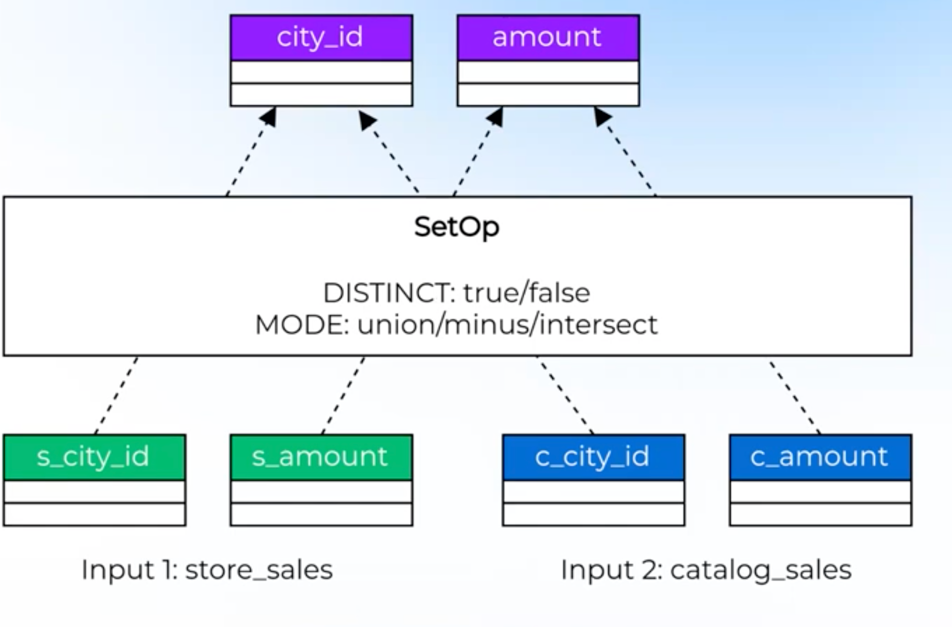
\includegraphics[width=\textwidth]{Pictures/Operators/Set}
            \caption{Работа Set}
        \end{minipage}
    \end{figure}

    \textbf{Set-оператор (Union, Minus, Intersect)} --- промежуточный оператор, производящий объединение/вычитание/пересечени данных из нескольких источников.

    \newpage

    \subsection{Пример перевода запроса в реляционные операторы}

    \begin{figure}[!h]
        \begin{minipage}{0.4\textwidth}
            \begin{lstlisting}[language=SQL,caption={Сложный запрос}]
                SELECT
                    dept,
                    SUM(salary) as sum_salary
                FROM employee
                WHERE city = MSK
                GROUP BY dept
                HAVING SUM(salary) > 1000
                ORDER BY SUBSTR (dept, 3) DESC
            \end{lstlisting}
        \end{minipage}
        \begin{minipage}{0.5\textwidth}
            \begin{lstlisting}[caption = {Реляционные операторы}]
                1. Scan [employee]
                2. Filter[city = MSK]
                3. Aggregate [groupingSet=[dept], SUM (salary)]
                4. Filter [sum_salary > 1000]
                5. Project [dept, sum_salary, $sort_col=SUBSTR(dept, 3)]
                6. Sort [$sort_col DESC]
                7. Project [dept, sum_salary]
            \end{lstlisting}
        \end{minipage}
    \end{figure}

    \newpage

    \subsection{Декларативная и императивная программы}

    \begin{lstlisting}[language=SQL]
        SELECT SUM(sales.amount )
        FROM sales JOIN city
        ON sales.city_id = city.id
        WHERE city.name = 'SPB'
    \end{lstlisting}

    \begin{itemize}
        \item \textbf{Декларативная прорамма}
        \begin{itemize}
            \item Сделать Join таблиц
            \item Применить фильтр
            \item Сделать аггрегацию
        \end{itemize}
        \item \textbf{Итеративная программа}
        \begin{itemize}
            \item Отсканировать таблицу city
            \item Вычислить city.id для подходящих под предикат строк, передать в sales
            \item Построить hash-таблицу для подходящих записей city
            \item Отсканировать sales, используя индекс по city\_id
            \item Многопоточно осуществить hash join и аггрегации
            \item Соединение результатов потоков
        \end{itemize}
    \end{itemize}

    \textbf{Задача:} оптимизация от декларативного исполнение к итеративному.
\end{document}